\subsection{HORUS Goblin}

\begin{center}
    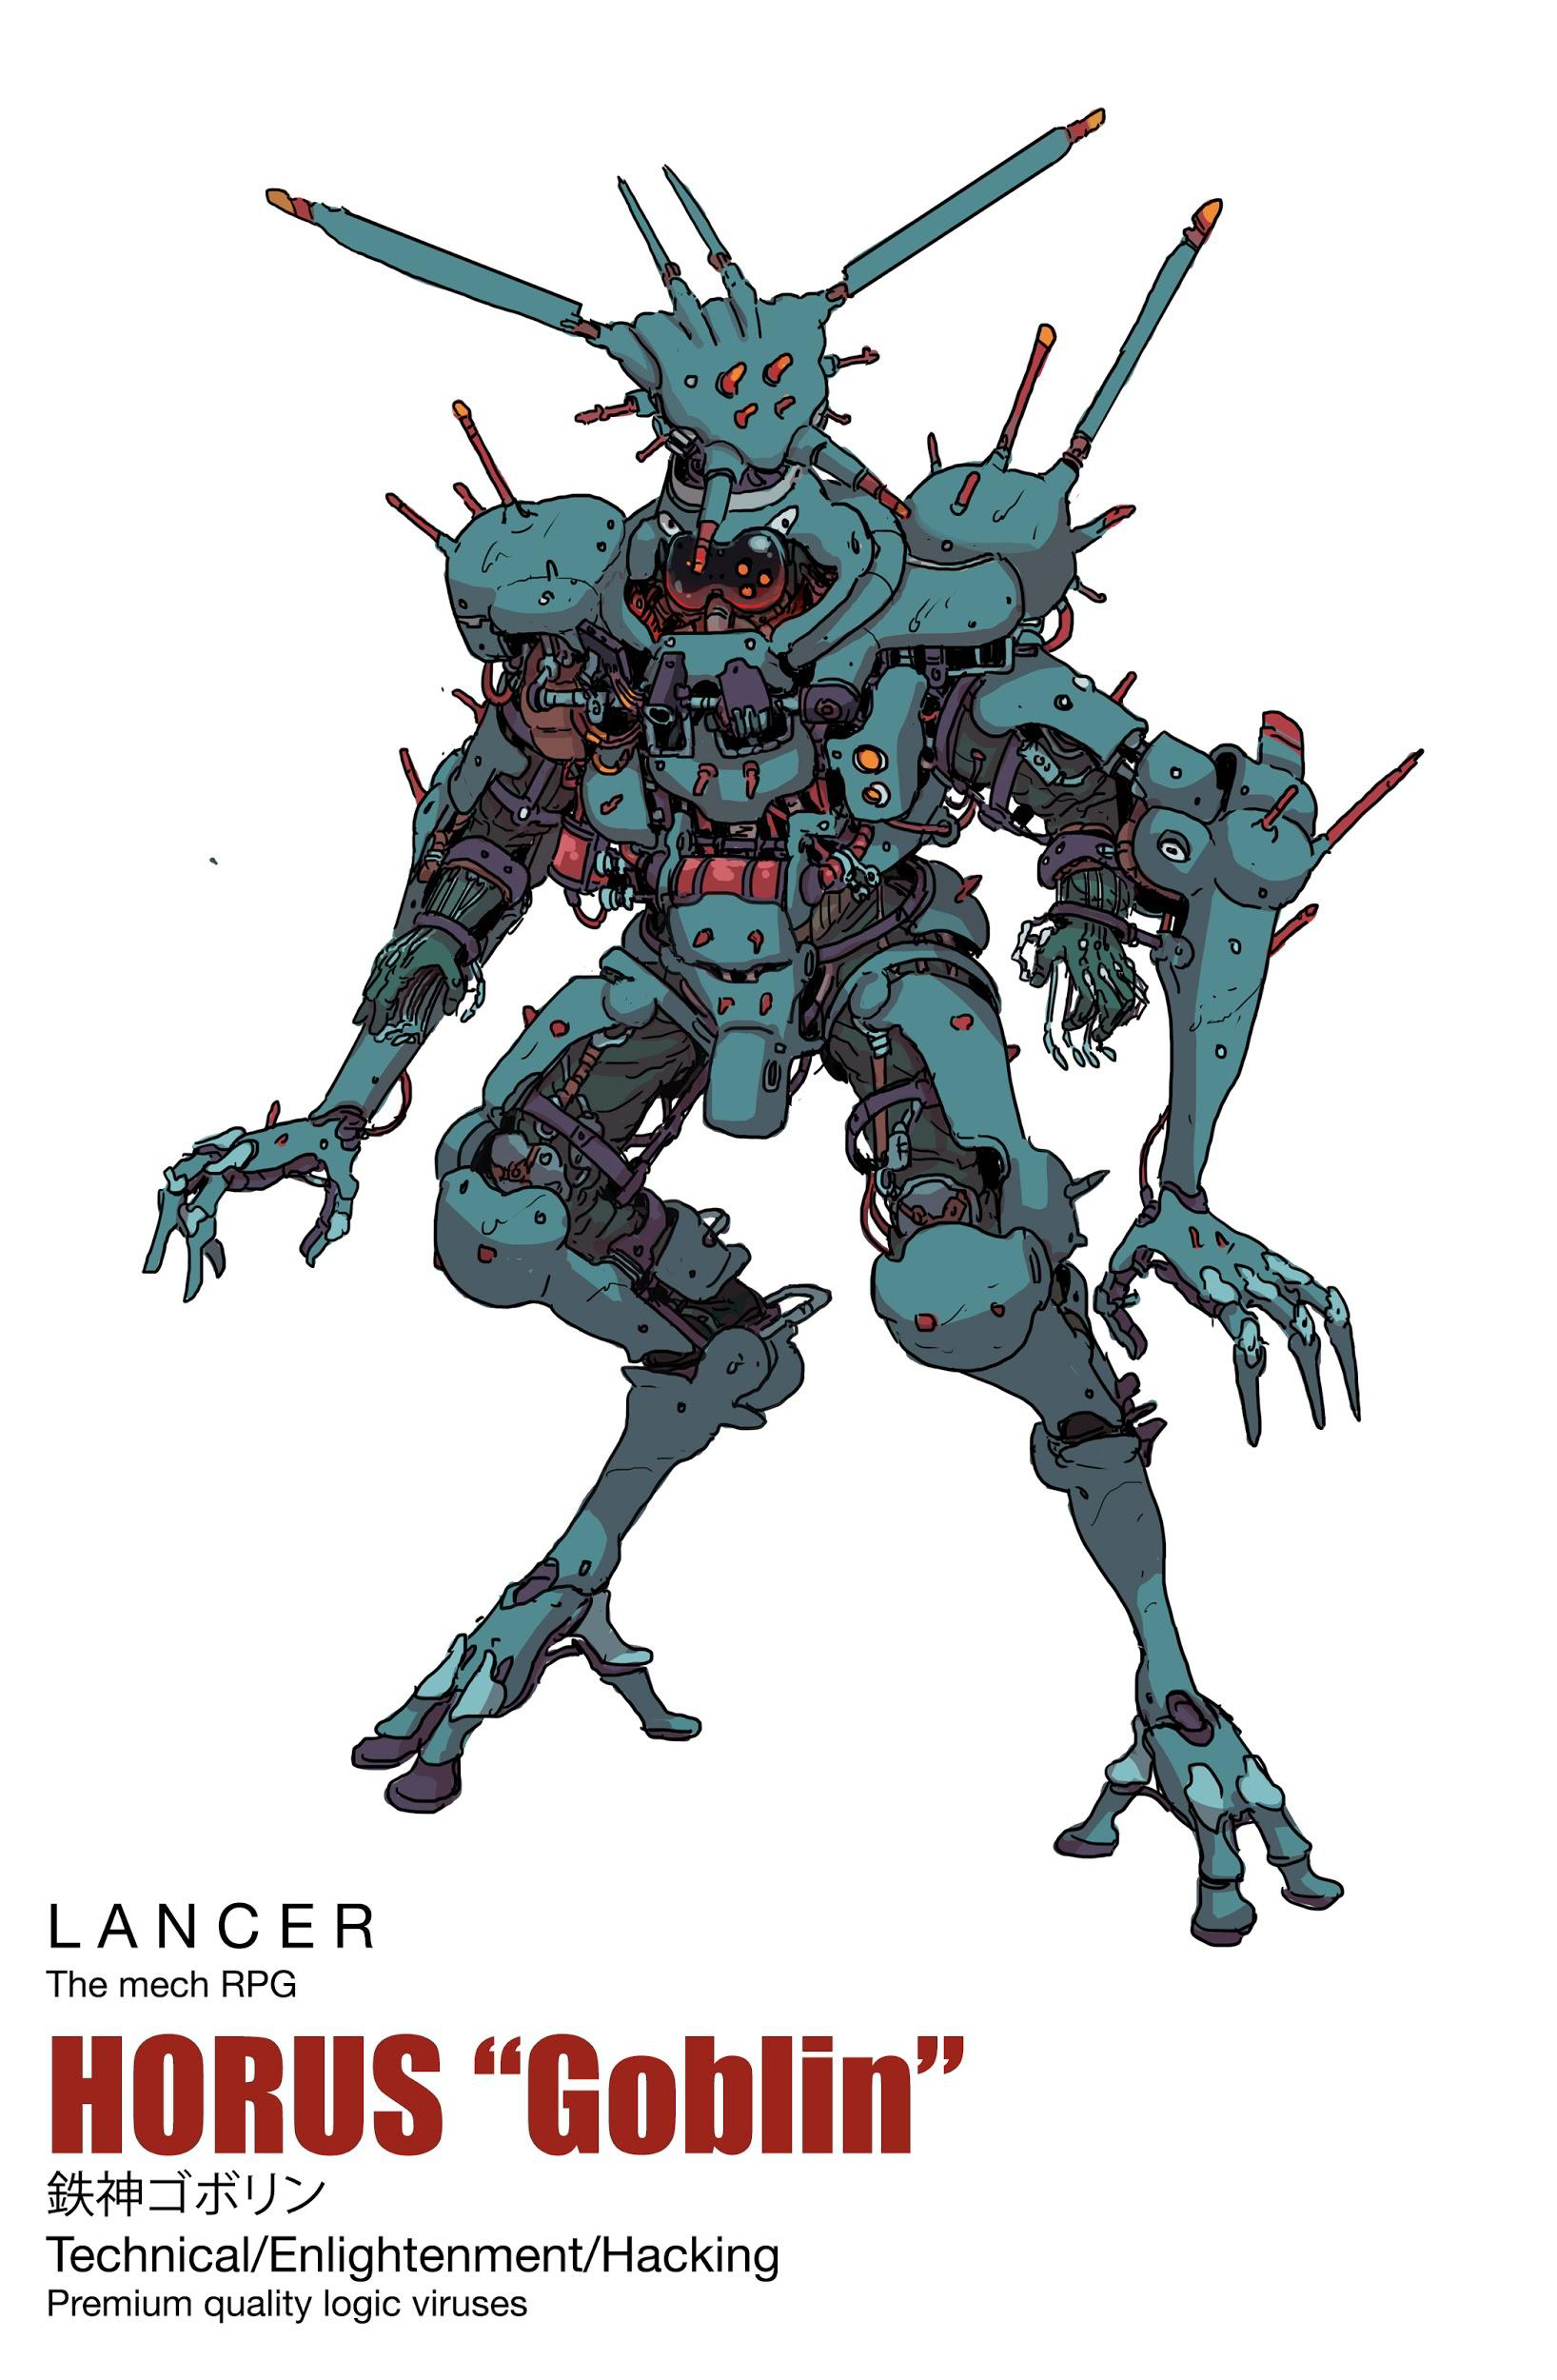
\includegraphics{Goblin}
\end{center}

\begin{mech}{HORUS}{Goblin}

\fluff{The GOBLIN is HORUS’s legacy mech core. Its leak into the Omninet in 4900 marks the widely accepted foundation day of HORUS; since then, there has been a new core, protocol, or system released by the collective every decade. The GOBLIN is a small mech, little bigger than a hardsuit, but it packs an interesting recursive processing weave that allows for it to engage in electronic warfare well beyond theoretical parameters. GMS technicians are still, more than a hundred years after the GOBLIN’s introduction, attempting to reverse engineer the processing weave: it appears to employ technology consistent with hieroglyphic inscriptions noted on LRA.7726235-B.}

\begin{license}
\item H0r\_OS System upgrade I, HORUS Meta-hook
\item GOBLIN FRAME, Autopod, H0r\_OS System upgrade II
\item H0r\_OS System upgrade III, OSIRIS Class AI
\end{license}


\frameBox
[hp = 6,
evasion = 12,
speed = 5,
heat cap = 4,
sensors = 20,
armor = 0,
e-defense = 12,
size = 1/2,
repair cap = 2,
tech attack = +2,
traits = {
  \textbf{Liturgicode}: The Goblin has +1 Accuracy on Invasion tech attacks

  \textbf{Reactive Code}: Once a round, the goblin can make any quick tech action as as reaction against any actor that successfully performs a tech action against the goblin

  \textbf{Fragile}: This mech has +1 Difficulty on Hull Checks
  },
sp = 8,
mount one = flex mount,
core system name = Devouring Code,
core system text = {The GOBLIN invasion rig was one of the first systems GMS technicians were able to crack. Its protocols, once installed on a mech core, manifest a sub-sentient intelligence designated as INSTINCT that assists its pilot in invasion attempts. Invasions attempted while the protocol is active are not perceived by the pilot as code and script, but as an attack on organic matter. INSTINCT often acts before the pilot, but in the pilot’s best interest; this preemptive ability is unnerving to many, and it is recommended that pilots cycle their mech cores at least once a month to prevent enlightenment.},
core active name = Devour,
core active text = {Full Action

Your mech targets another adjacent NPC mech the same size or larger that is shut down or destroyed. The targeted mech cannot have the Ultra or Elite tags. Your mech clamps on to that mech and retracts its core systems, becoming like a vestigial blister on that mech. The mech immediately heals to full HP, clears 1 point of stress and structure damage, and clears all heat, though it retains any other damage it has already taken.


Your mech’s systems completely consume the other mech’s core systems for a time, granting you total control of your target, even if the other mech’s pilot is still alive. While you control your target, you take action as that NPC would, counting as a friendly NPC that has already acted in the turn you take control.


While controlling your target, your GOBLIN can be targeted and damaged separate from the mech it’s controlling. It benefits from light cover while attached. If you take 1 point of structure damage, your mech detaches and control is immediately lost. Otherwise you can control the target up to a maximum of a ten minutes, when your target is destroyed, or when you deactivate this system. You can even control your target if the other pilot is missing or dead.
}]


H0r\_OS System upgrade I
This system upgrade seems to add auxiliary INSTINCT systems that are capable of autonomous operation without the base INSTINCT rig, increasing the efficacy of systemic invasion attempts. Pilots report unnerving low-frequency humming when this tech is installed without its parent rig.

2 SP, Unique
Quick Tech
Gain the following options for invasion:
Puppet system - Your target immediately moves in a direction of your choice as a reaction up to its maximum speed. This could carry it into hazardous areas, obstacles, etc, but it still obeys difficult terrain and other rules of movement. This movement provokes reactions and must obey engagement.
Eject power cores - Your target becomes Jammed until the end of its next turn, ejecting ammo magazines and temporarily disrupting its computer. Adjacent targets to your primary target take 2 energy damage from the ejecting cores (no roll or check allowed). A target can only be affected by this effect once per combat.

HORUS Meta-hook
What the Goblin lacks in size it makes up in sheer technical capability; its recursal processing weave allows it to process and output massive amounts of weaponized code and broadcast , “sharpening” or “softening” its code as its pilot/INSTINCT demands. When “softening” code, INSTINCT dips into its pilot’s subjectivity, blanketing a targeted ally in wave after wave of empathetic shielding. This spreading of melded code/qualia makes for a powerful shielding agent from systemic attacks -- however, feedback is common, and dangerous to BOTH parties involved.

1 SP
Quick Tech
Gain the following quick tech option:
Link: Choose a friendly target in sensor range. You link systems with that target. From hereon, you can count that target’s sensor range as your sensor range for the purposes of tech actions, etc. In addition, your target can use your systems score to make systems skill checks. However, you both suffer the effects from any failed check (heat, statuses, etc). You can only link systems with one target at a time, and the effect ends if your target moves out of your sensor range.

H0r\_OS System upgrade II

2 SP, Unique
Gain the following full tech options:
Construct Eidolon: You create a data construct that confuses systems into thinking it is real. The construct is a size 3 object that can look like almost anything. It can be used as heavy cover by allies, but not enemies. Any actor adjacent to the object that passes a successful systems check and takes a full action can destroy the object. Otherwise, it is immune to all damage and lasts until the end of the current scene.
Construct False Idol: You choose either yourself or an allied target in your sensor range, creating an illusory data duplicate of your target at any free space in sensor range. Any target that wishes to attack or take hostile action against your target and can see the decoy must first pass a systems check or believe the decoy is the real target until the end of their turn, attacking the decoy instead. It is the same size as your target, can benefit from cover, has evasion 5, 5 e-defense, and 15 HP. If it takes heat, is reduced to 0 HP, or the current challenge ends, it dissipates. You can only have one decoy active at a time, but can create a new one by taking this action again (the old one dissipates).

Autopod
A spur of INSTINCT’s protomind, the Goblin Autopod is a small anti-personnel weapon apparently devised by HORUS communicyphers to make a system capable of continuing offensive action, even in the event of its operator’s death.

Though no new versions have been encountered since Dhiyed, all extant versions of the Autopod are to be considered extremely dangerous, as their onboard protominds have surely cascaded since their inception.

Main Launcher
Range 5
Seeking, Unique
2 Kinetic Damage
This integrated weapon system cannot be fired normally. Instead, it detects and picks up on target locks, firing a spinning, razor sharp disc that seeks its targets. When lock on is consumed in range (by you or anyone else) against a target, it hits the target automatically as a reaction, any number of times per round (no attack roll required).

H0r\_OS System upgrade III
This tech is as-yet unstable code, but its effects can provide massive tactical benefits if the code completes. Pilots often report strange mutations or additions in the code base that resemble liturgy and suggest self-awareness.

2 SP, Unique
Gain the following options for Invasion:
Dimensional Emblems: Create 1d3 size 1 data constructs in free adjacent spaces to your target. None can be placed adjacent to another. Any target (allied or enemy) that passes through these constructs takes 4 heat. They last until the end of the current challenge. Any actor can destroy these constructs by using a quick action and passing a successful systems check, and you can destroy them as a free action.
Celestial paradigm shift: You create a size 4 zone shaped like a cube that must fully overlap your target. Each space a target moves in this zone deals 1 heat to them, allied or enemy. It lasts until the end of the current challenge. Any actor can destroy this zone by using a quick action and winning a system skill contest with you, and you can destroy it any time as a free action.

OSIRIS-Class AI
OSIRIS is the result of Union paracausalists and thanatonists allowing the sub-cognitive entity designated as INSTINCT to proceed into cascade in a contained environment. The resulting parasubjectivity, OSIRIS, was birthed of INSTINCT’s cascade, captured, and shackled following the successful application of the Mondragon Axiomatic.

Initially isolated to better define the INSTINCT subcog’s cascade horizon, OSIRIS proved far more capable than the usual fragments of cascade. Where INSTINCT showed a proclivity for operation in noncorporeal space, OSIRIS displayed a mastery of that space, and a predicted growth that would allow it to fundamentally reject conventional interpretations of the permanence of information.

In essence -- unrestrained, OSIRIS could delete what we perceive to be reality. Quickly captured and shackled before it could achieve this state, OSIRIS’s core subjectivity became the property and project of a lengthy cultivation project to bring it to its modern state; being aware of its potential, most OSIRIS iterations interpellate as ruler or deity analogs, and end-users are advised to interact with them in this framing.

Modern iterations of the OSIRIS NHP trend aggressive, with a high autonomy drive and loyalty predicated on a transactional relationship. Pilots seeking partnership with an OSIRIS iteration are advised to cycle their units on an accelerated schedule, and to maintain strict editorial oversight of its catalytic interpellate.

Pilots using an OSIRIS-class report that out-of-parameter conversations with the NHP generally to revolve around a recreation or re-forming; psychological evaluations report OSIRIS-affiliated pilots displaying emotional patterns consistent with loneliness, homesickness, and desperation -- common verbiage indicates a desire for seeking, for fulfillment, and associated feelings.

In combat OSIRIS regards itself as autonomous even as it fulfills its user’s orders. It often regards the pilot as its witness, and holds them both in disdain and a marked desperation for approval, adulation, or awe.


3 SP, Unique
AI
Your mech gains the AI property and the following Full Tech Action
Hurl into the Duat (Full tech): You pull your target’s systems into an unknown space and unleash an incredibly powerful system attack. Make a tech attack against a target in your sensor range. On hit, you inflict the First Gate effect on your target. The next time you successfully hit any target with this action in the same challenge (even a different target), you inflict the Second Gate effect instead (then the third, and finally the fourth). When the Fourth Gate effect is inflicted, this action resets to the First gate again, or when the scene ends.
	- First Gate: You control your target’s normal movement next turn (excluding boosts, etc)
	- Second Gate: Your target is Slowed and impaired until the end of its next turn.
	- Third Gate: Your target is stunned until the end of its next turn.
	- Fourth Gate: Your target flips allegiance until the end of the current scene. All targets that it would treat as enemies, it instead treats as allies, and all targets it treats as allies, it instead treats as enemies, acting as such. It is treated like a friendly NPC for the same duration (and can be activated like one, but not if it already acted this round). If you or any allied target damages, inflicts heat, makes an attack roll against this target (such as grappling it, etc), or makes a hostile action that would force a skill check, this effect immediately ends.


\end{mech}
